\documentclass[a4paper,10pt]{article}
\usepackage[utf8]{inputenc}
\usepackage{listings}
\usepackage{color}
\usepackage{url}
\usepackage{hyperref}
\usepackage{graphicx}

\definecolor{grey}{rgb}{0.9,0.9,0.9}

\lstset{
language=Python,
basicstyle=\footnotesize\fontfamily{pcr},
backgroundcolor=\color{grey},
numbers=left,
numberstyle=\tiny,
numbersep=5pt,
showstringspaces=false,
tabsize=3,
breaklines=true
}

%opening
\title{Karger's Mincut}
\author{Abdeselam El-Haman Abdeselam}

\begin{document}
\sloppy
\maketitle


\section{Analysis}

Karger's algorithm is a Montecarlo algorithm that estimates an answer to the mincut problem.
The algorithm contracts edges randomly until there is only 2 vertices in the graph, then it's a cut.

The probability that the algorithm succeeds is of $\frac{2}{n(n-1)}$. This bound can be improved to at least$1 - \frac{1}{e}$ by repeating the
algorithm $\frac{n^2}{2}$ times.

This algorithm then has been tried with 3 distinct graphs.
The first one is the famous \href{https://en.wikipedia.org/wiki/Zachary's_karate_club}{Zachary's Karate Club}
The second one is a "supervertex" graph where it simulates a simple graph where every node is a $K_x$ subgraph.\ref{supervertex}
The third one will be a graph composed by 2 $K_x$ subgraphs connected by $x-2$ edges, building so a minimum
cut between the 2 subgraphs.

\begin{figure}[h]
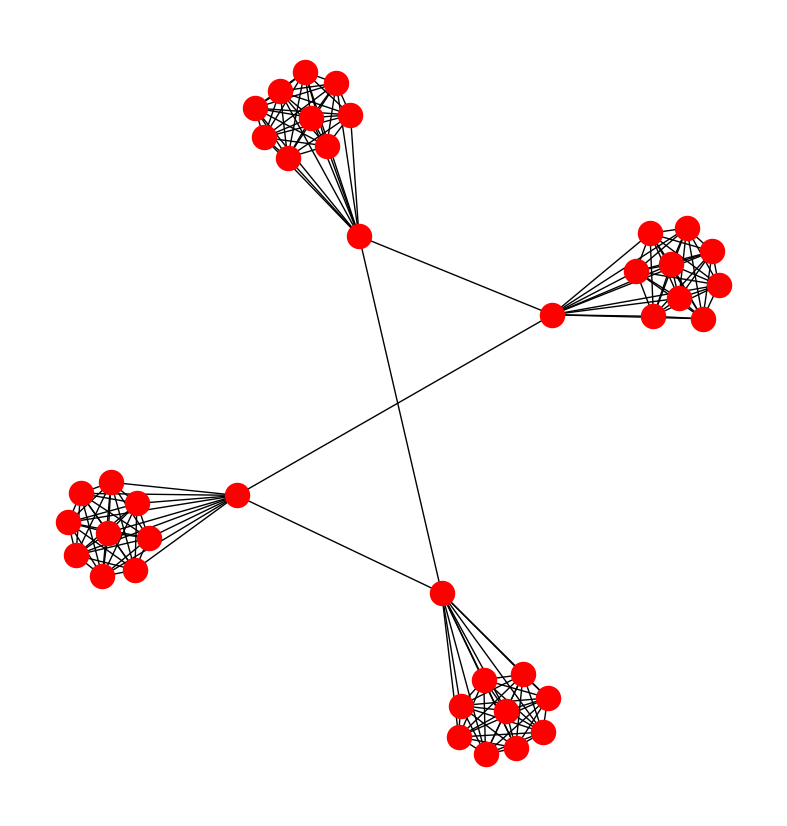
\includegraphics[width=\linewidth]{graph2}
\caption{The "supervertex" graph}
\label{supervertex}
\end{figure}

\section{Implementation}

This algorithm has been developed using the \href{https://networkx.github.io}{networkx library}.
I've chosen to use this library because it has an absolute abstraction of graphs and it implements already
the edge contraction. It has also \href{https://networkx.github.io/documentation/stable/reference/generators.html}{graph generators} to
create graphs from a lot of different kind of graphs.

Networkx also has an implementation of mincut-maxflow to find the minimum edge cut, so I've used it to check the results afterwards.

\section{Results}

For each graph we've computed the Karger algorithm $\frac{n^2}{2}$ times, to check the $\frac{1}{e}$ factor.

The first observation is that for every graph, the percentage of success in average is:
\\

\begin{tabular}{ | l | c | }
  \hline
  Karate Club & $65\%$ \\
\hline
  Supervertex & $84\%$ \\
  \hline
  Double $K_x$ & $1\%$ \\
  \hline
\end{tabular}
\\

We can see here that there's a little percentage of success in the graphs where the relation between
the size of the minimum cut and the size of the graph.
Then 100 tests have been done with that number of repetitions and for each one the results are 100\% succesful.
So the above $1-\frac{1}{e}$ of success is not only correct but also 100\% correct for the graphs
that I've chosen.
To have better results, we should have a bigger graph with bigger cuts, but for that
we'd need a better CPU.

\end{document}
